\emph{Finite-Difference-Time-Domain (FDTD) Method for Random Lasing Simulations}
As our third application study we use a simulation from the field of optical physics, where the propagation of light through a medium is simulated.

In the simulation two fields, the electric field $\vec{E}$ and the magnetic field $\vec{H}$, are iteratively updated using stencils computations.
The Maxwell's equations are the basic equations describing electrodynamic processes in nature and are used here to describe the light propagating through a non-magnetic (\emph{dielectric}) medium.

\bigskip
\begin{minipage}{.44\linewidth}
\begin{equation} \vec{\nabla}\vec{E}\left(\vec{r}, t\right) = 0, \label{eq:div_e}\end{equation}
\end{minipage}
\hspace{.04\linewidth}
\begin{minipage}{.44\linewidth}
\begin{equation} \vec{\nabla}\vec{H}\left(\vec{r}, t\right) = 0, \label{eq:div_h}\end{equation}
\end{minipage}

\bigskip

\begin{minipage}{.44\linewidth}
\begin{equation} \frac{\partial\vec{H}\left(\vec{r}, t\right)}{\partial t} = -\frac{1}{\mu_0}\vec{\nabla} \times \vec{E}\left(\vec{r}, t\right), \label{eq:rot_h}\end{equation}
\end{minipage}
\hspace{.04\linewidth}
\begin{minipage}{.44\linewidth}
\begin{equation} \frac{\partial\vec{D}\left(\vec{r}, t\right)}{\partial t} = \frac{1}{\epsilon_0}\vec{\nabla} \times \vec{H}\left(\vec{r}, t\right), \label{eq:rot_d}\end{equation}
\end{minipage}
\bigskip

\newpage
\noindent
Eq. (\ref{eq:div_e})-(\ref{eq:rot_d}) show the Maxwell's equations consisting of four coupled partial differential equations (PDEs).
To couple the polarisation of a medium $\vec{P}$ to the electric field, Eq. (\ref{eq:flussdichte}) is introduced:

\begin{equation}
\vec{E}\left(\vec{r}, t\right) = \frac{\vec{D}\left(\vec{r}, t\right) - \vec{P}\left(\vec{r}, t, \vec{N}\right)}{\epsilon_0\epsilon_r\left(\vec{r}\right)}
\label{eq:flussdichte}
\end{equation}

\noindent
Here $\vec{N}$ is the induced energy distribution in the medium using the model proposed in~\cite{Jiang2000}.
The parameters $\mu_0$, $\epsilon_0$ and $\epsilon_r$ describe the permeability and permittivity of free space and the relative permittivity of the dielectric medium.

To solve this set of coupled PDEs, the Finite-Difference-Time-Domain Method (short FDTD)~\cite{Yee1966} can be used.
Here we use a form of FDTD where the electric and magnet field are discretized within a n-dimensional regular grid.
$\vec{E}$ and $\vec{H}$ are shifted against each other by a half grid-cell.
This allows the calculation of the new values by computing finite differences between two values of the grid.
Using the FDTD method, we implemented a simulation of the effect of random lasing on a nano-meter scale~\cite{Cao1999} for our evaluation.

Figure \ref{fig:fields} shows a visualization of the electric field (and the field intensity) after about  $1\,ps$ of simulation time equal to $60\,000$ iterations.
The shown field distribution can be found also in~\cite{Cao2000, Sebbah2002, Yamilov2005}.%, however the simulation parameters are different.

\begin{figure}[t]
	\begin{minipage}[b]{.48\textwidth}
    \centering
	  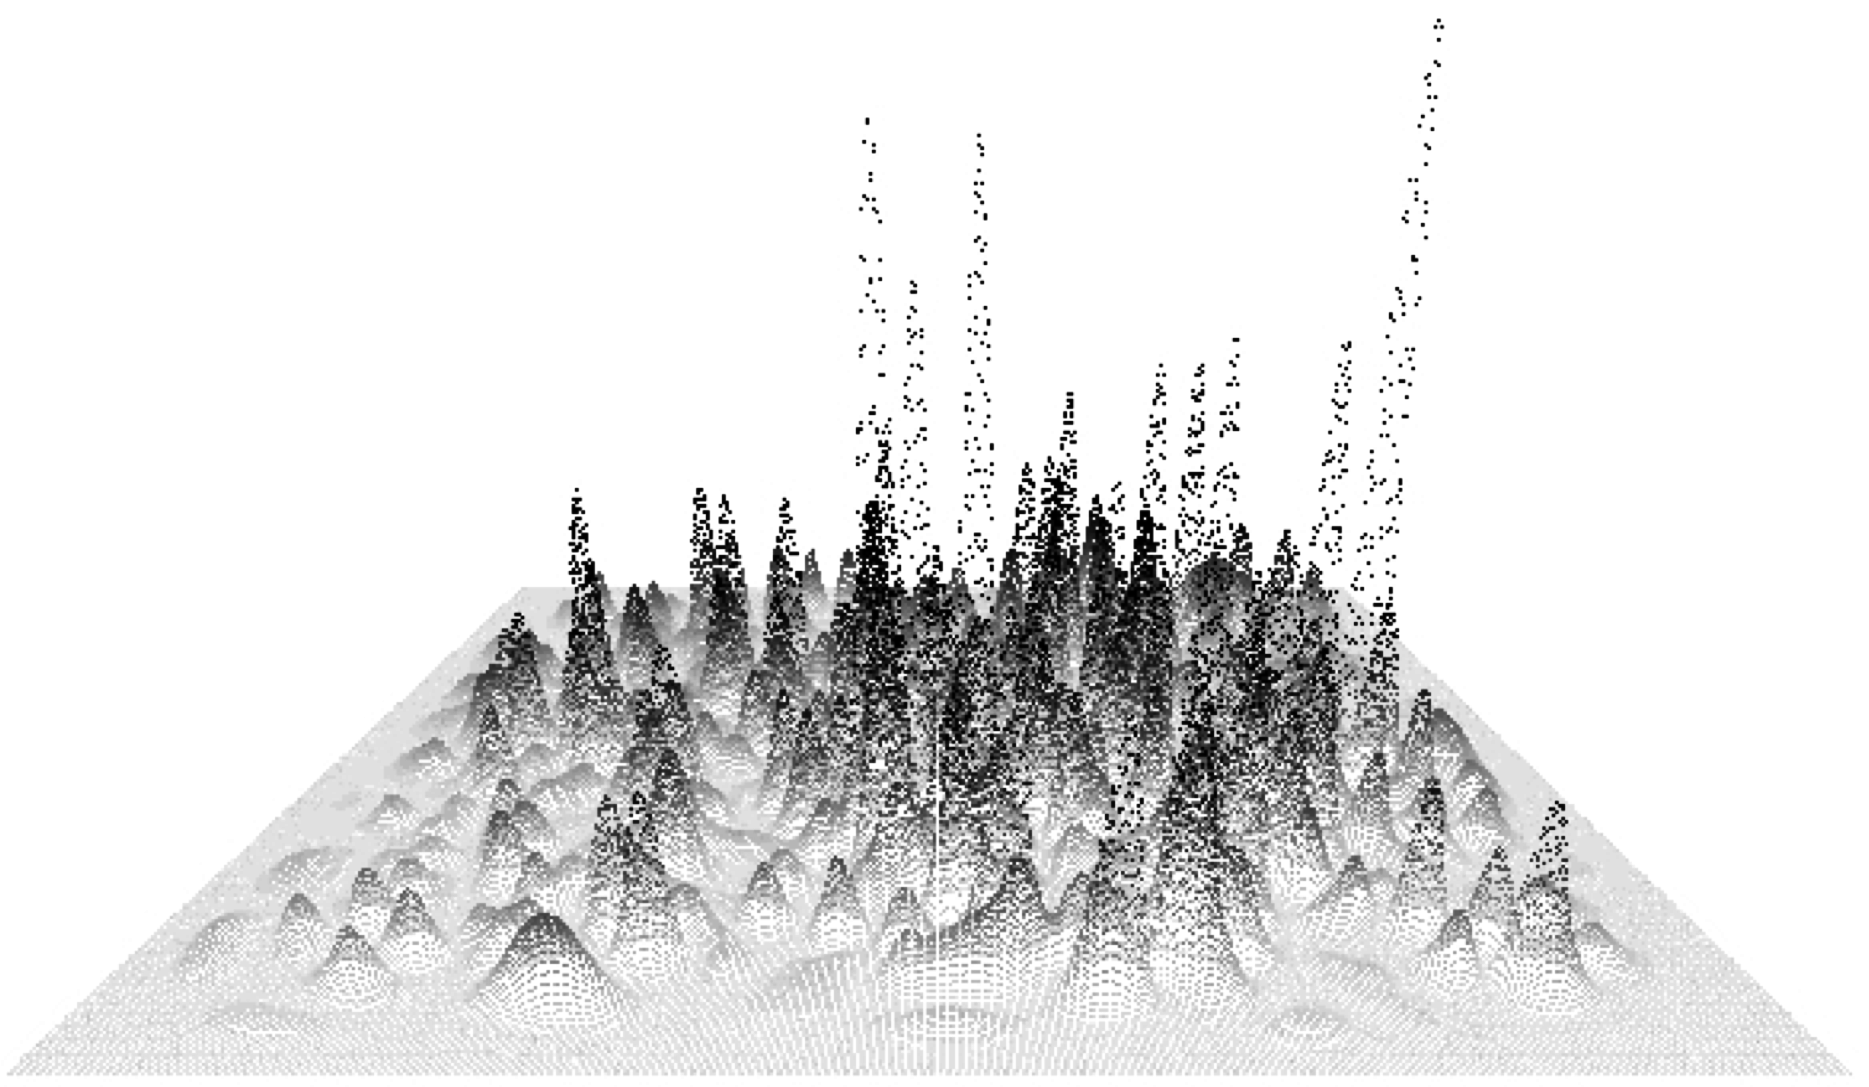
\includegraphics[width=\textwidth]{PPL/rl3.png}
  	\caption{\small The image shows a 3D representation of the intensity for the 2D electric field as computed by the SkelCL FDTD implementation after $60\,000$ iterations.}
	  \label{fig:fields}
  \end{minipage}
  \hspace{.02\textwidth}
  \begin{minipage}[b]{.48\textwidth}
    \centering
	  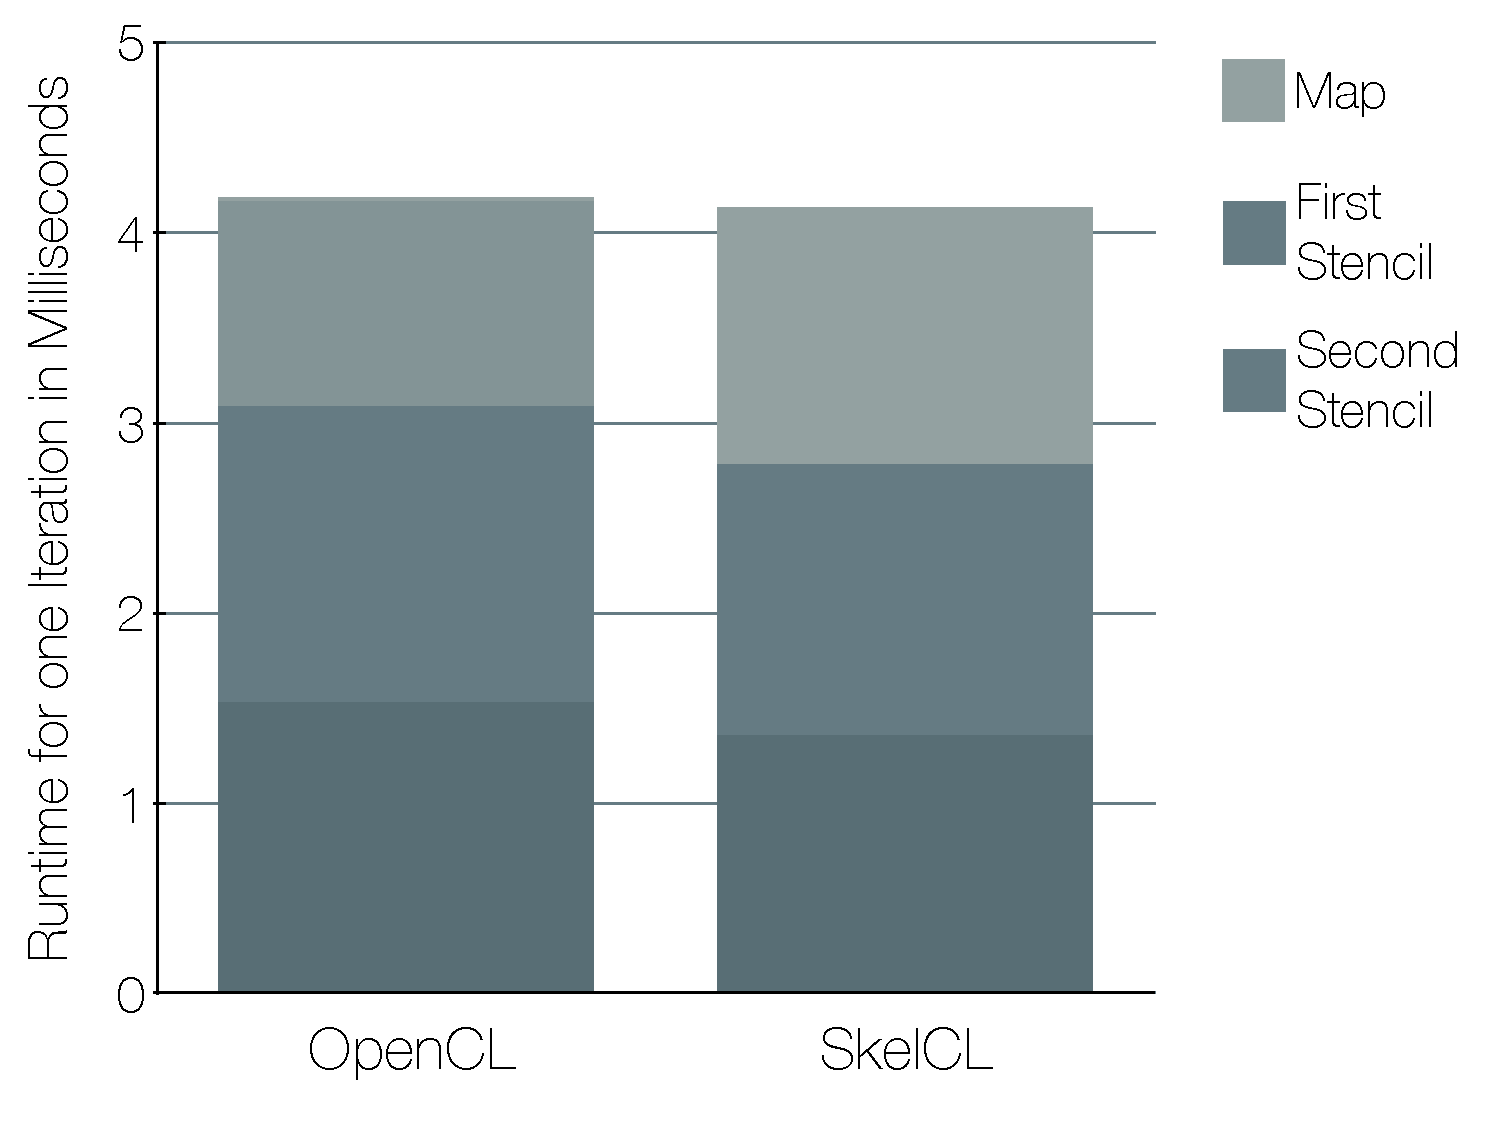
\includegraphics[width=\textwidth]{PPL/fdtd.pdf}
  	\caption{\small Runtime for one iteration of the FDTD application.}
  	\label{fig:fdtd_eval}
  \end{minipage}
  \bigskip
\end{figure}

\begin{figure}[tbp]
\begin{lstlisting}[%
  caption={Source code of the FDTD application in SkelCL},%
  label={lst:fdtd}]
Map<float4(float4)>     updateEnergyDist(...);
Stencil<float4(float4)> updateEField(...);
Stencil<float4(float4)> updateHField(
  "float4 func(float4_matrix_t E, float4_matrix_t H) { ... }");

Matrix<float4> N; // energy distribution in the medium
Matrix<float4> E; // E (electric) field
Matrix<float4> H; // H (magnetic) field

for (...) { // for each iteration
  updateEnergyDist(out(N), N, out(E));  
  updateEField(out(E), H, E);
  updateHField(out(H), E, H); }
\end{lstlisting}
\end{figure}

We implemented a two-dimensional version using SkelCL as well as a manually tuned OpenCL implementation.
To solve the PDEs (\ref{eq:rot_h}) and (\ref{eq:rot_d}), two separated three-point stencil computations are performed and one map computation for the gain-model is necessary.
Eq. (\ref{eq:div_e}) and (\ref{eq:div_h}) are implicitly solved by the FDTD method~\cite{Yee1966}.
Listing~\ref{lst:fdtd} shows the SkelCL code of the application:
in every iteration first the energy distribution is updated (line 11) using a map skeleton (defined in line 1);
then the first stencil (defined in line 2) updates the electric field $\vec{E}$ by combining a single element of $\vec{E}$ with three elements of the magnetic field $\vec{H}$ (line 12);
and finally the second stencil (defined in line 3) updates $\vec{H}$ by combining a single element of $\vec{H}$ with three elements of $\vec{E}$ (line 13).

Please note that the two stencil computations require both fields ($\vec{E}$ and $\vec{H}$) as input.
To implement this, we use the \emph{additional argument} feature of SkelCL which allows the additional field to be passed to skeletons on execution (see line 12 and 13).
The additional arguments are passed unchanged to the customizing function of the skeleton, therefore, the function customizing the stencil in line 4 now accepts $\vec{H}$ as a second parameter.
This feature greatly increases the flexibility of applications written in SkelCL.

In the evaluation we used a $2048 \times 2048$ sized matrix with a spatial resolution of $100$ cells per $\mu m$. 
This matrix corresponds to a square-shaped medium with the edge length of $20.1\,\mu m$. 
The medium size is actually smaller than the matrix size because of the border handling. 
To provide a physically correct simulation, the borders of the magnet field must be treated specially.
The Stencil skeleton provides sufficient functionality to allow for such border handling in the computation code.


We compared our SkelCL based implementation to a handwritten, fine-tuned OpenCL implementation which is based on \cite{Knitter2013}.
The OpenCL version is specifically designed for modern Nvidia GPUs.
In particular, it exploits the L1 and L2 caches of the Nvidia Fermi and Kepler architecture and does not explicitly make use of the local memory.
We performed the experiments on a system with a modern Nvidia K20c Kepler GPU with 5GB memory and 2496 compute cores.
Figure \ref{fig:fdtd_eval} shows the median times of a simulation time of $1\,ps$ equal to 60\, 000 iterations.
The SkelCL version slightly outperforms the OpenCL version by $2\%$.
The two stencil skeletons achieve ${\sim}10\%$ faster runtimes than the corresponding OpenCL kernels but the map skeleton is ${\sim}20\%$ slower, because it reads and writes all elements exactly once, while the customized OpenCL kernel does not write back all elements.
For this application it seems beneficial to make direct usage of the local memory as our implementation of the Stencil skeleton does, instead of relying on the caches of the hardware, as the OpenCL implementation does.

% This application study shows that real-world applications written in SkelCL can achieve the performance competitive with manually written OpenCL code.
